\section{本研究的意义和目的}
基于视频的人体运动姿态分析有着广阔的引用场景,因此其吸引了越来越多研究者的兴趣。其应用领域主要表现在以下几个方面:

\textbf{虚拟现实和增强现实:}在虚拟环境中,人与虚拟角色进行的动作模拟,可以通过基于视频的人体姿态运动分析,给参与者提供更多的交互形式。计算机可以从视频中获取人体运动数据,可以使我们用新的虚拟人物或者动画角色替换原始视频中的人物,得到更好的效果。

\textbf{智能人机交互:}智能人机交互是指让目前的计算机摆脱键盘鼠标等传统交互设备的局限,通过人体运动等更为自然的方式直接用人类进行交互,使得计算机能像人与人之间的交流一样更自然便捷。这要求计算机能够更进一步地从面部表情、语言、身体动作去分析人的行为,而基于视觉分析的技术能够在语言干扰大的环境下提供更准确的输入。

\textbf{电影制作:}目前计算机进行电影和动画制作时,人物角色的动作、姿态的设计主要来源于运动捕捉设备的使用。传统的运动捕捉设备需要在人体身上贴满标签,该方法成本较高,使用麻烦。而基于视频的人体运动动作的获取,将给人体动画和游戏提供更加丰富的数据,并且也能大大降低运动捕捉系统的成本,提高制作效率。


\textbf{健康监护:}在临床上,通过获取患者的行走动作,利用计算机来分析其运动数据,有助于判断身体某部分的受伤情况或者畸形程度,从而帮助做出有效的治疗手段。而传统的运动分析系统大多采样专用的视频设备和计算机设备,价格昂贵,操作复杂,使用过程具有较高的专业性,因此不适合进行大范围的推广,难以在普通医院使用。因此采用普通电脑连接普通摄像机的人体运动姿态分析系统有着更广阔的应用场合和前景。

\textbf{智能安防监控:}目前监控摄像机在公共场所已经广泛存在,但是无法发挥其实时、积极的作用,大多数场合只能通过专门的工作人员监视显示器,以发现异常的事件。或者将监控视频保存,出现异常情况时,才调用监控记录进行查看,而这样又会占用大量存储设备,因此无法保留长时间记录。如果通过视频进行监视,通过计算机进行实时分析,通过检测并跟踪其中的人体运动,分析人体行为,当有异常情况发生时,系统能够及时警报,从而有效防止此类事件的发生。同时也可以减少大量雇佣人员的成本,以及购买存储设备的成本。

\begin{figure}[ht] \centering
    \subfigure[AR场景] { \label{fig:a}
    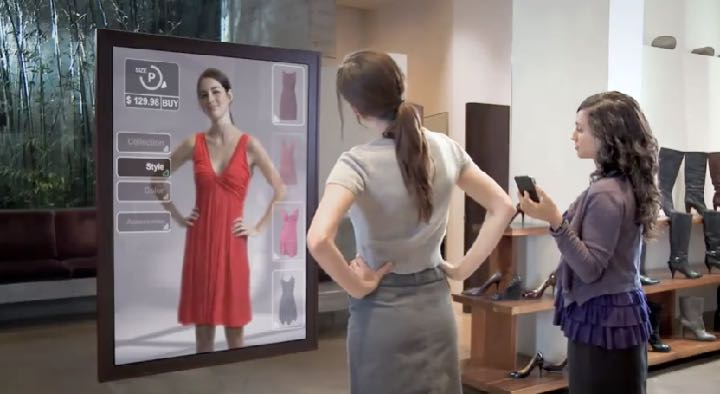
\includegraphics[height=0.15\columnwidth]{figure/background/ar.png}
    }
    \subfigure[人机交互] { \label{fig:b}
    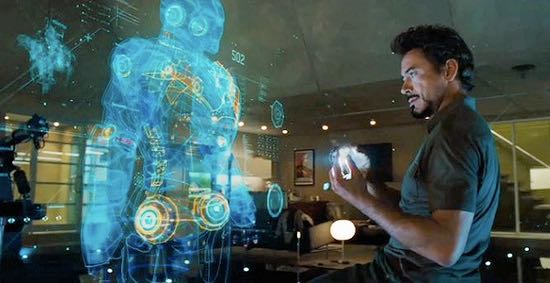
\includegraphics[height=0.15\columnwidth]{figure/background/hcl.png}
    }
    \subfigure[电影制作] { \label{fig:b}
    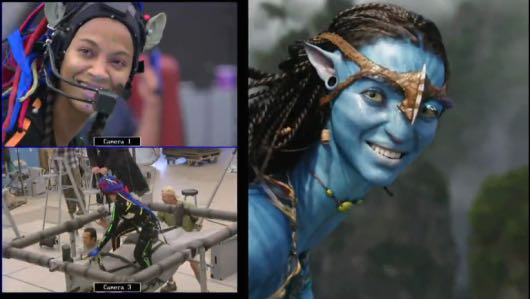
\includegraphics[height=0.15\columnwidth]{figure/background/movie.png}
    }
    \subfigure[娱乐游戏] { \label{fig:b}
    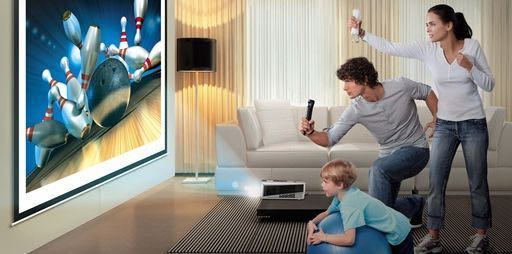
\includegraphics[height=0.15\columnwidth]{figure/background/gaming.png}
    }
    \subfigure[健康监护] { \label{fig:b}
    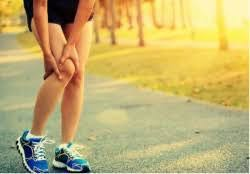
\includegraphics[height=0.15\columnwidth]{figure/background/health.png}
    }
    \subfigure[安防监控] { \label{fig:b}
    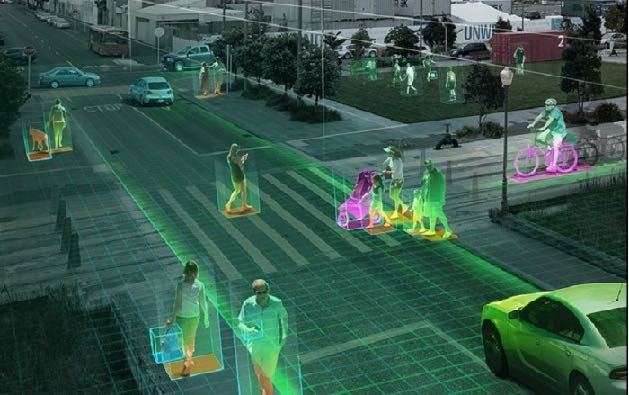
\includegraphics[height=0.15\columnwidth]{figure/background/surveil.png}
    }
    \caption{应用场景}
    \label{fig:appli}
\end{figure}

\begin{figure}[ht]
    \centering
    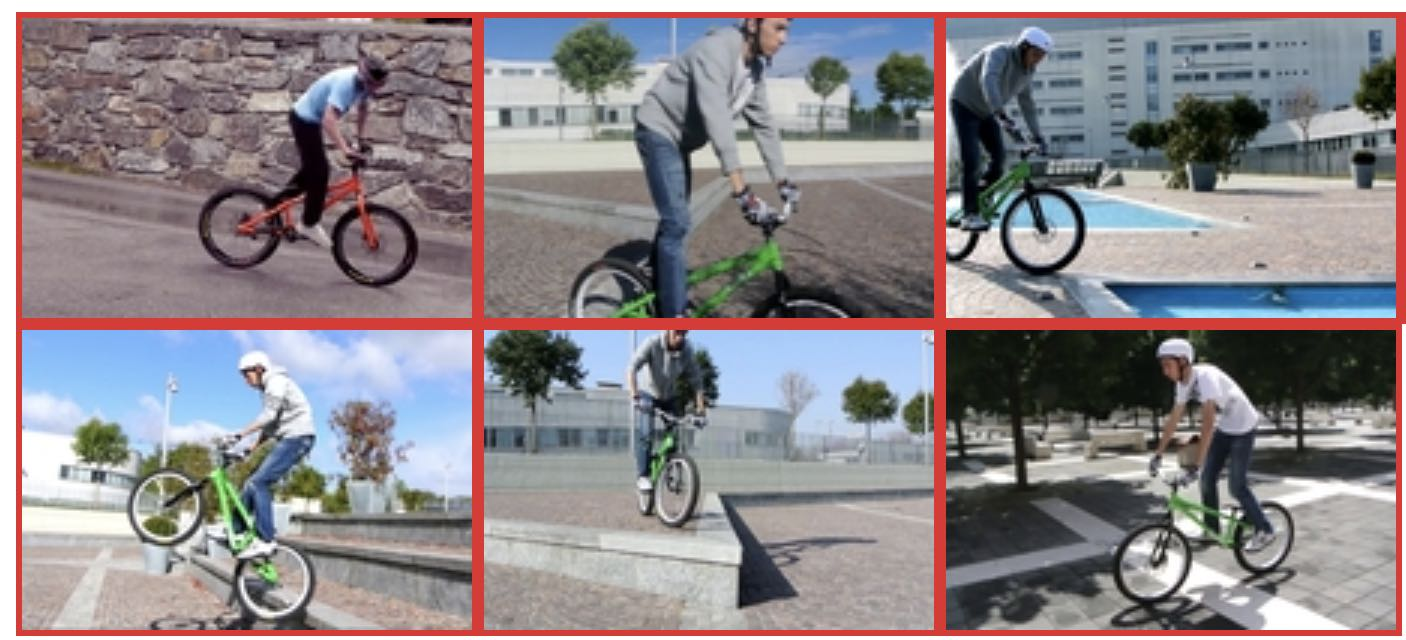
\includegraphics[width=.8\linewidth]{background/cha1}
    \caption{\label{fig:cha1}面临的挑战:外观差异}
\end{figure}

\begin{figure}[ht]
    \centering
    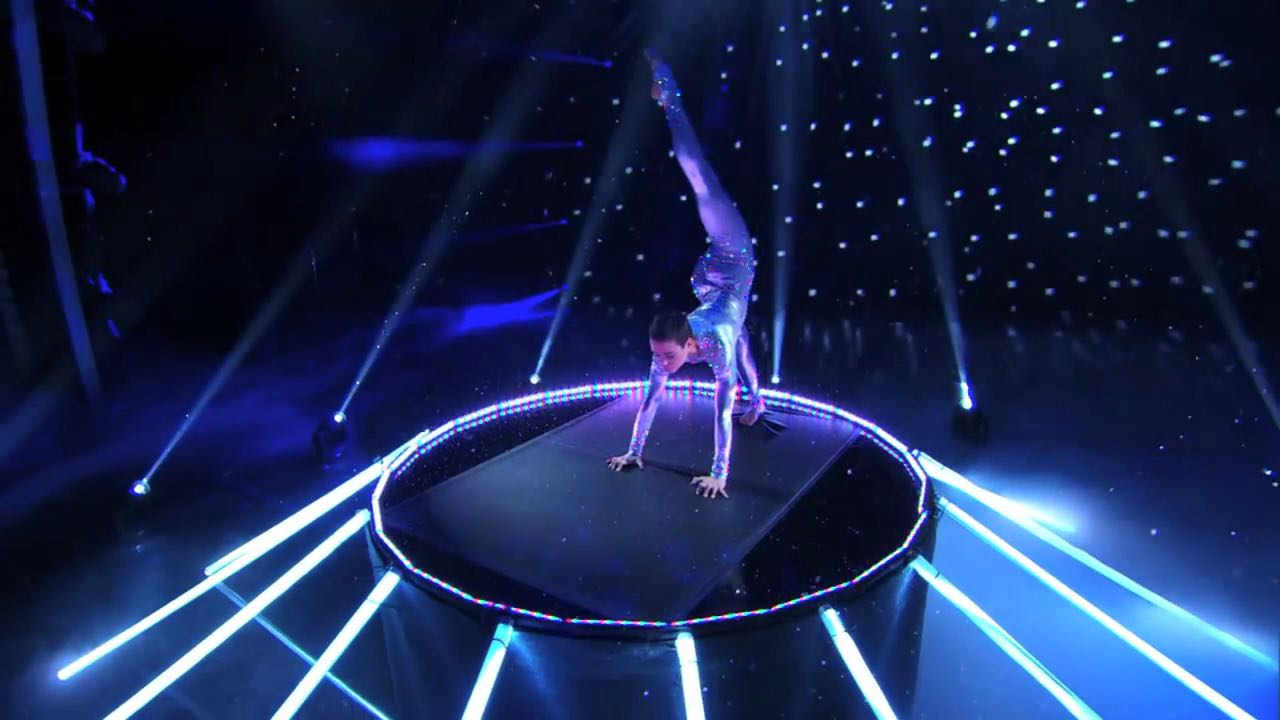
\includegraphics[width=.8\linewidth]{background/cha2}
    \caption{\label{fig:cha2}面临的挑战:姿势差异}
\end{figure}

\begin{figure}[ht]
    \centering
    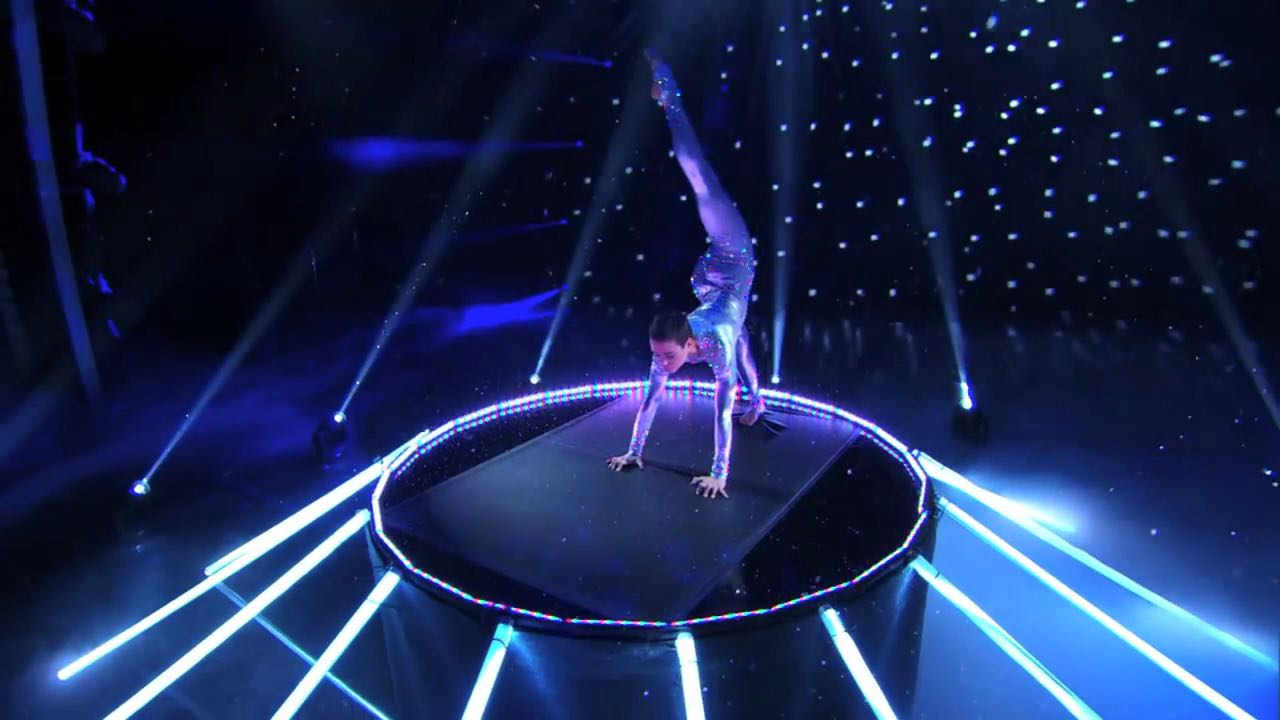
\includegraphics[width=.8\linewidth]{background/cha2}
    \caption{\label{fig:cha3}面临的挑战:单目导致的歧义-缺图}
\end{figure}

\begin{figure}[ht]
    \centering
    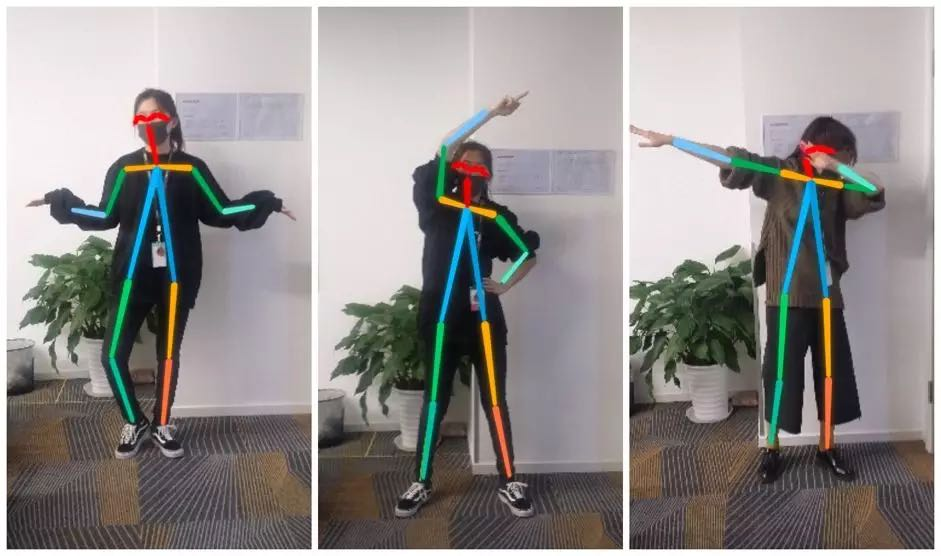
\includegraphics[width=.8\linewidth]{background/human}
    \caption{\label{fig:cha3}二维人体姿态估计}
\end{figure}

\section{主要研究内容}

\section{技术路线}

\subsection{数据集}

\subsection{人体检测}

\subsection{二维人体姿态估计}

\subsection{三维人体姿态估计}

\subsection{三维人体模型估计}


\section{课题研究进展}
